\begin{appendices}
\chapter{Static ahead of time thread and core partitioning}
This section shows the performance distribution graphs for all the benchmarks explored in Chapter~\ref{chp:streamit}.
The curves represent the density distribution for different core compositions as a function of the number of threads.
The right hand side Y-axis represents the number of threads present in the current version of the benchmark whilst the left Y-Axis represents the density normalized by the total number of points in the design space.
For each of the threaded versions the benchmark runs using 100 different core-compositions.
The density curve for thread 15 is a single point as there exists only a single composition, so a line is drawn to represent where that point lies.
\begin{figure}[t]
\center
 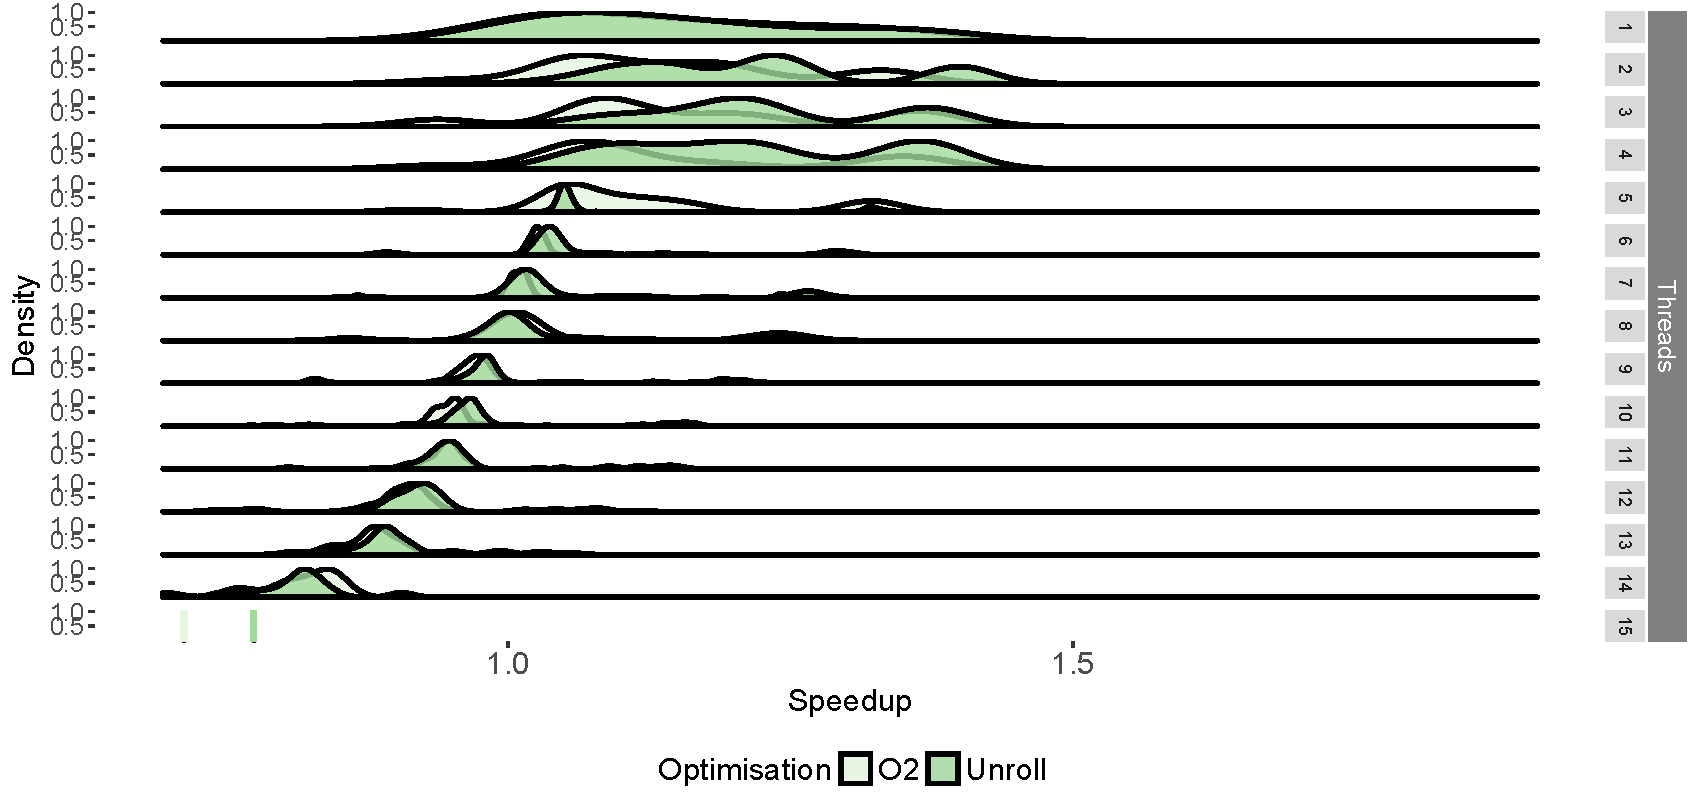
\includegraphics[width=1\textwidth]{streamit-paper/graphics/appendixgraphs/audio_total2.pdf}
\caption{Audio}\label{chp:stream:at}

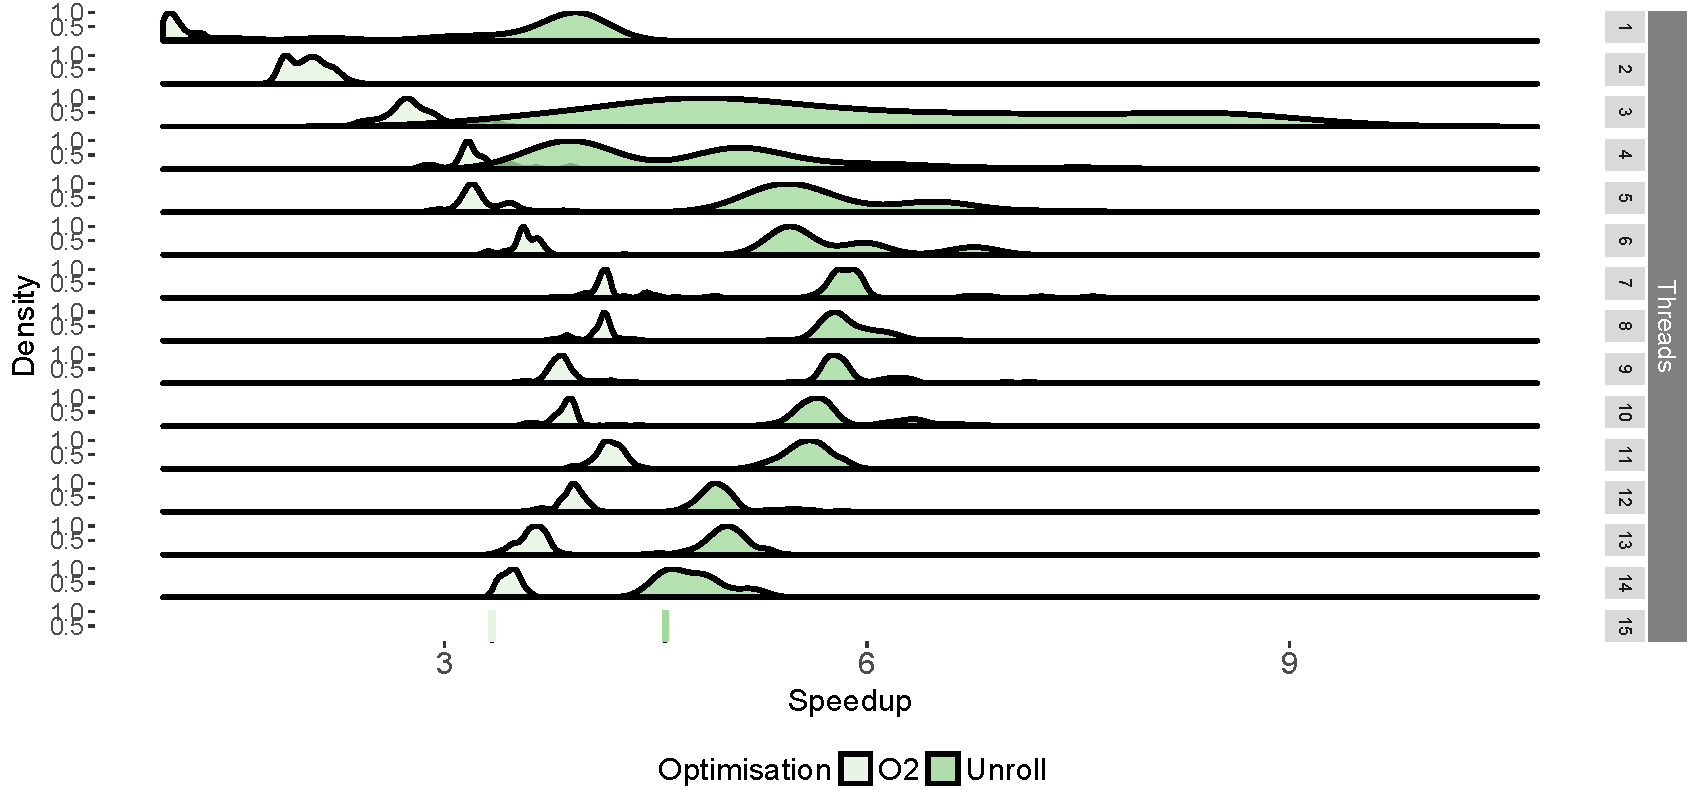
\includegraphics[width=1\textwidth]{streamit-paper/graphics/appendixgraphs/beamformer_total2.pdf}
\caption{Beam}\label{chp:stream:bt}

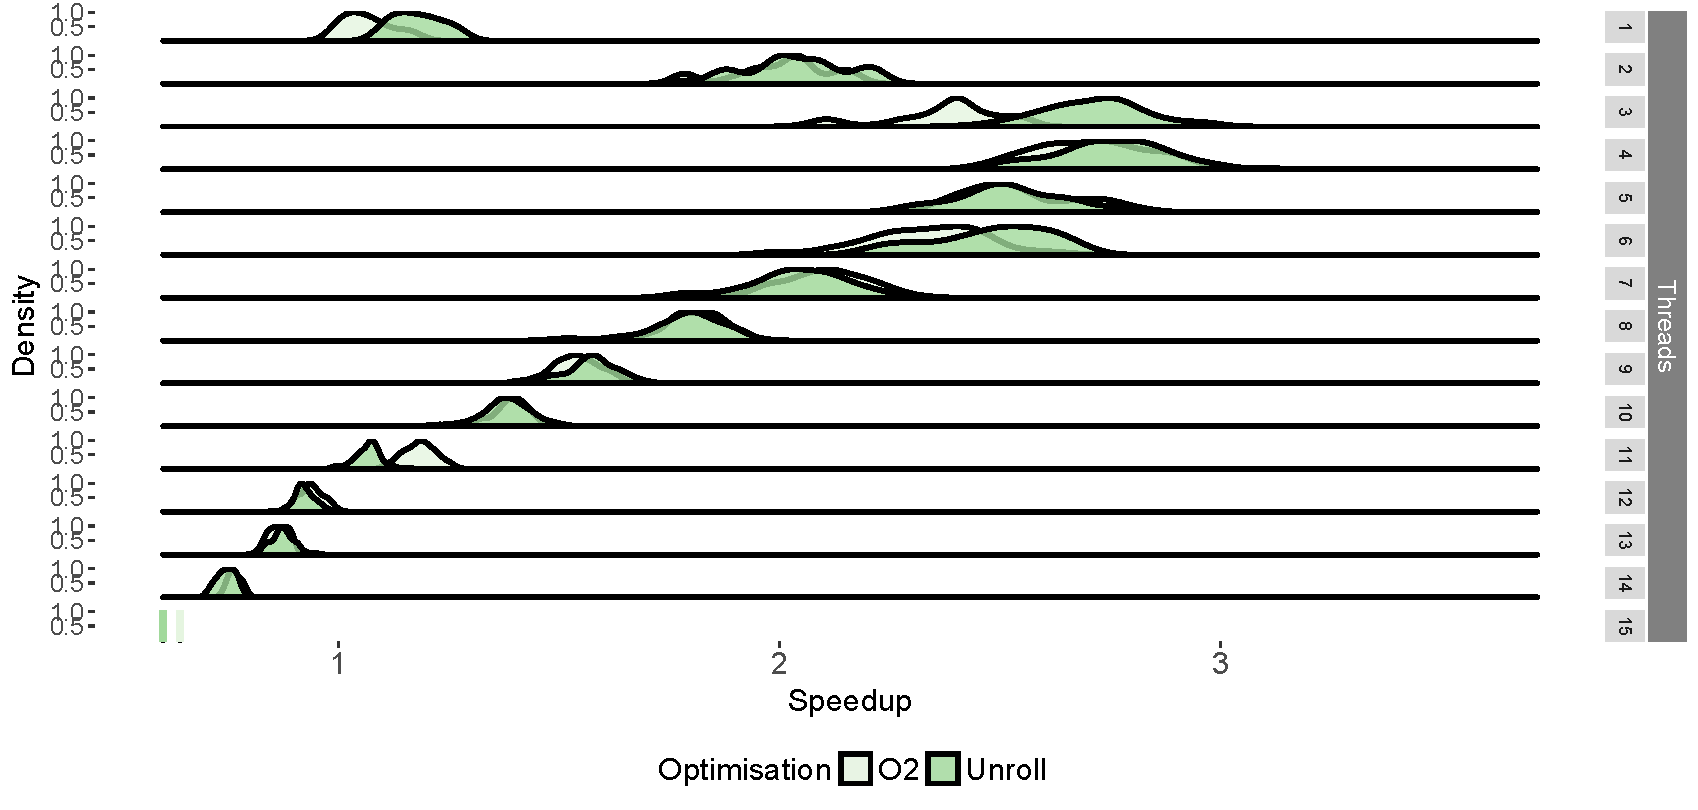
\includegraphics[width=1\textwidth]{streamit-paper/graphics/appendixgraphs/bitonic-total2.pdf}
\caption{Bitonic}\label{chp:stream:bt2}
\end{figure}

\begin{figure}[t]
\center
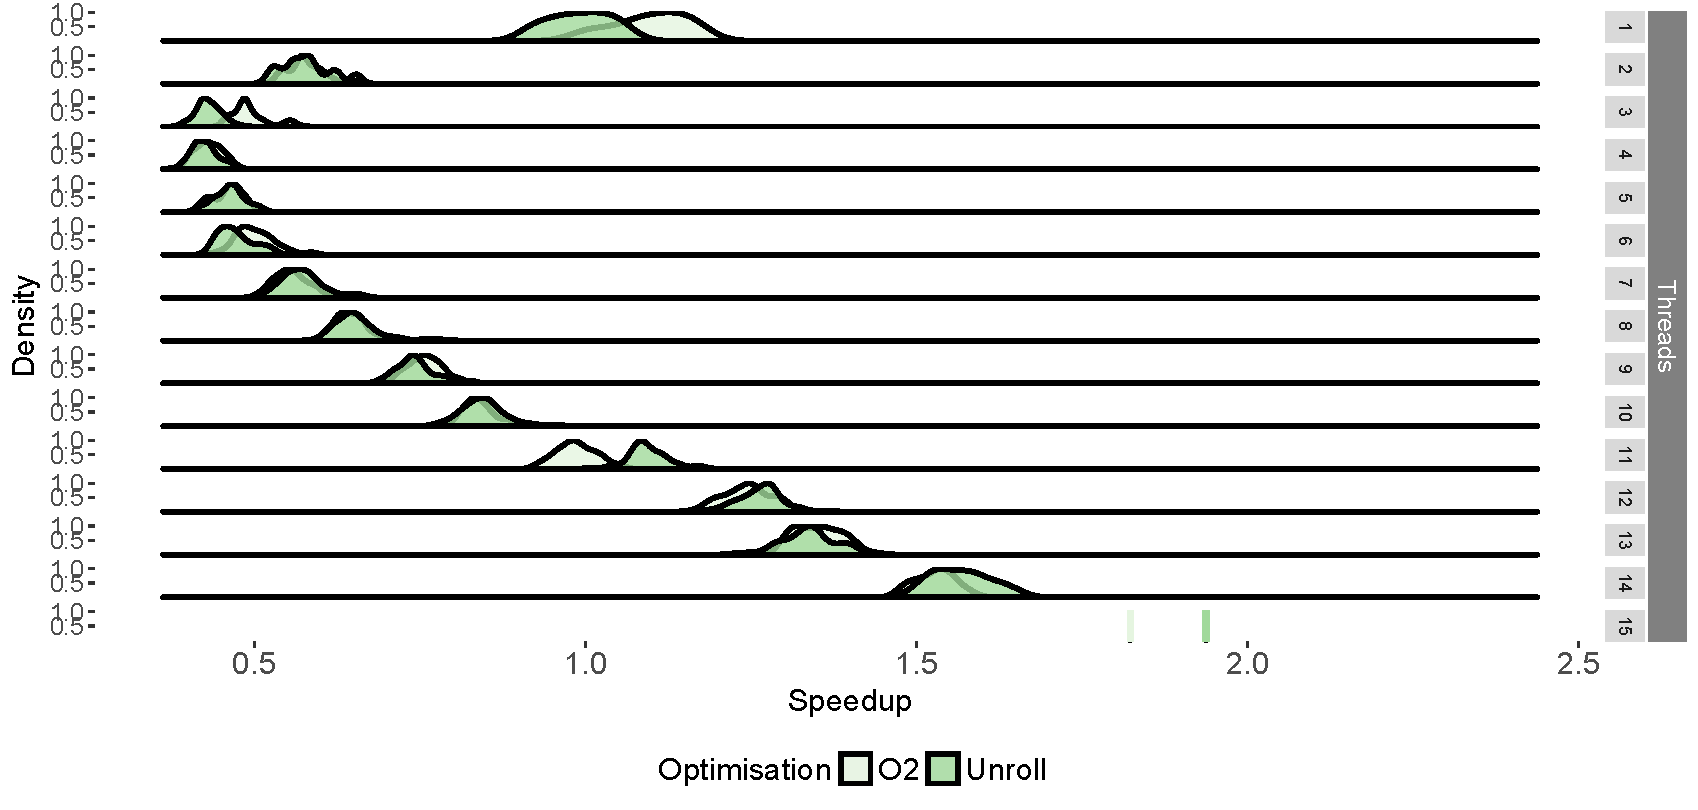
\includegraphics[width=1\textwidth]{streamit-paper/graphics/appendixgraphs/bubble-total2.pdf}
\caption{Bubble}\label{chp:stream:bt3}
\center
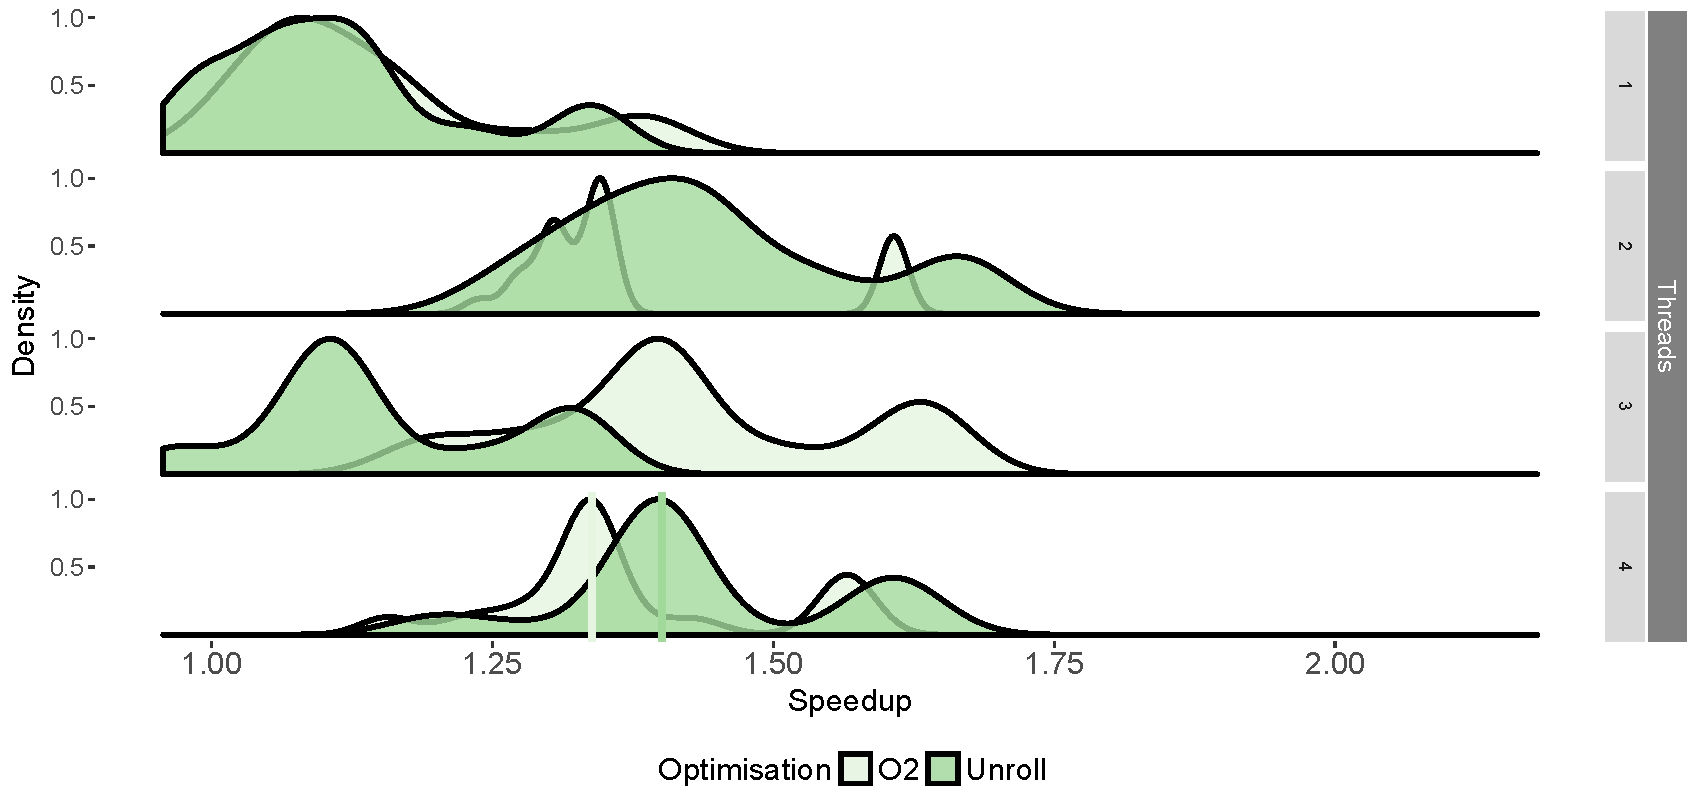
\includegraphics[width=1\textwidth]{streamit-paper/graphics/appendixgraphs/cfar-total2.pdf}
\caption{CFAR}\label{chp:stream:ct}
\center
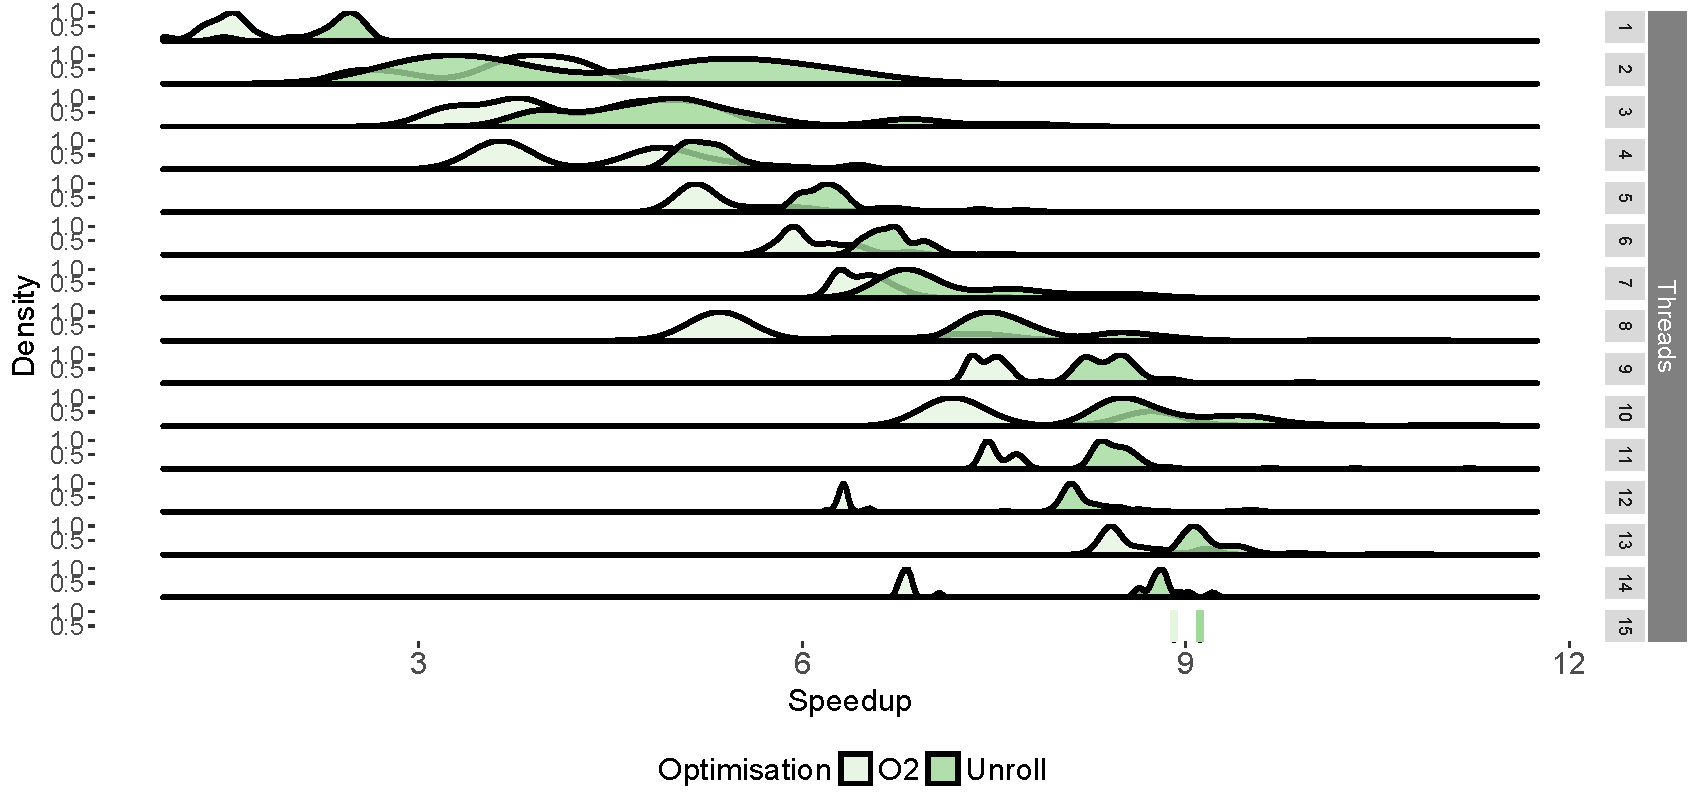
\includegraphics[width=1\textwidth]{streamit-paper/graphics/appendixgraphs/channel-total2.pdf}
\caption{Channel}\label{chp:stream:ct2}
\end{figure}
\begin{figure}[t]
\center
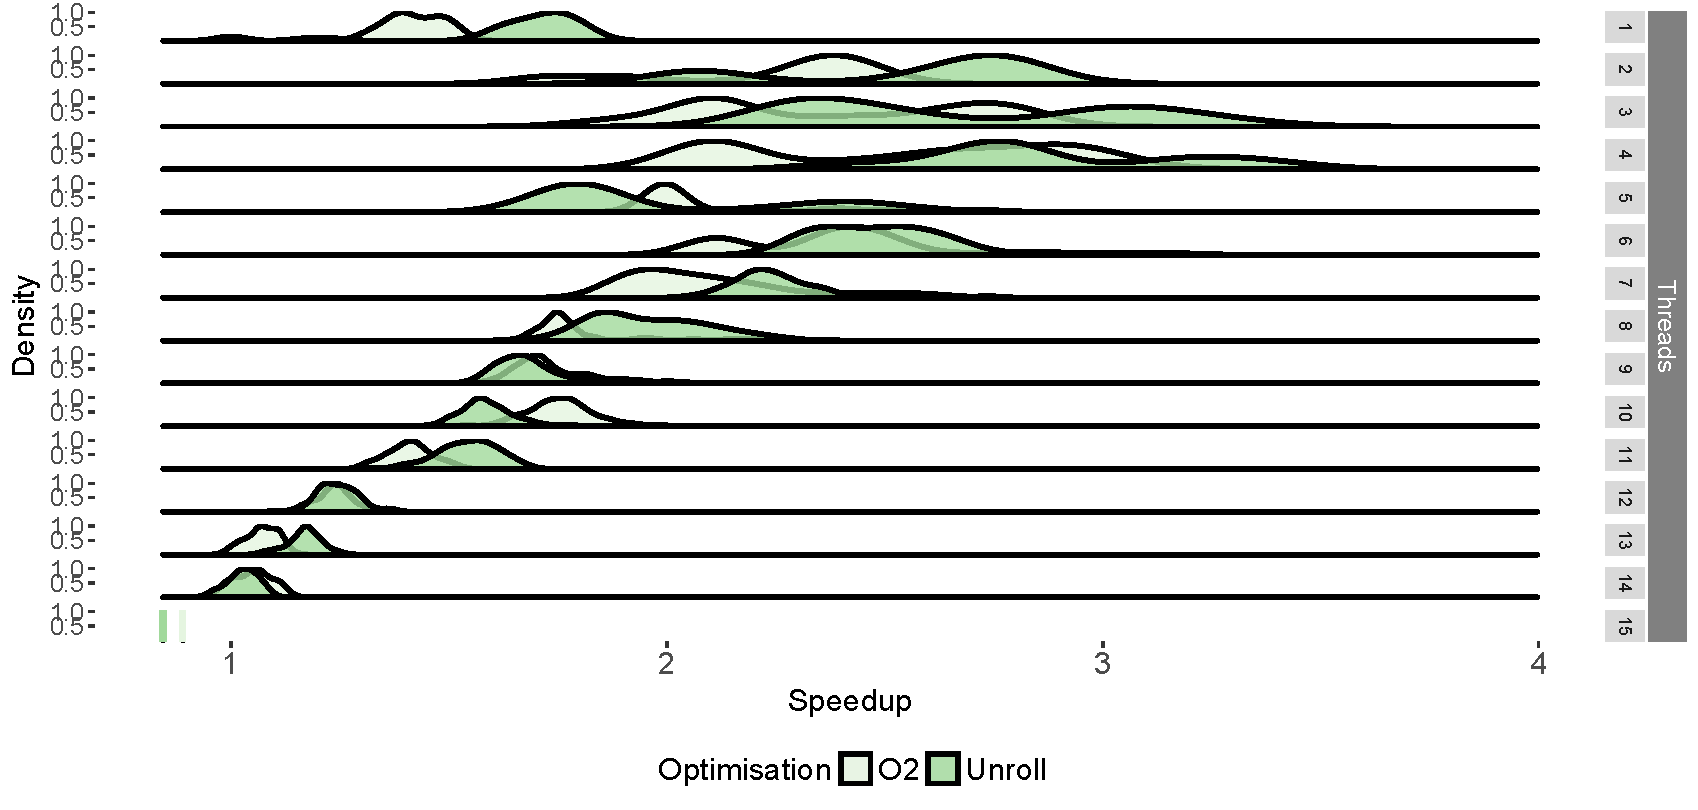
\includegraphics[width=1\textwidth]{streamit-paper/graphics/appendixgraphs/fft-total2.pdf}
\caption{FFT}\label{chp:stream:ft}
\center
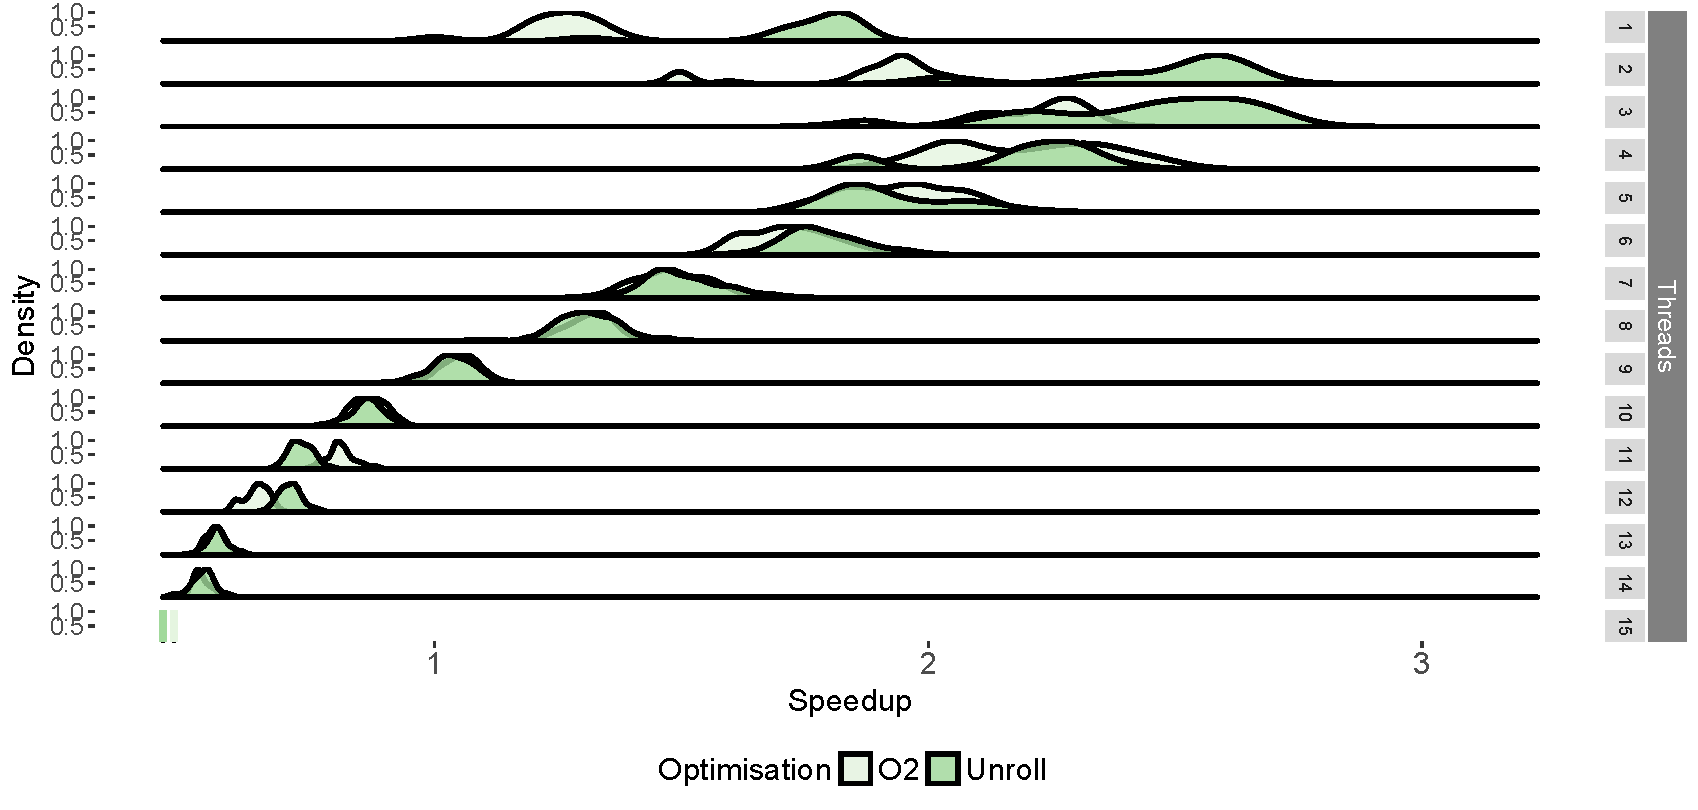
\includegraphics[width=1\textwidth]{streamit-paper/graphics/appendixgraphs/fft3-total2.pdf}
\caption{FFT3}\label{chp:stream:f3t}
\center
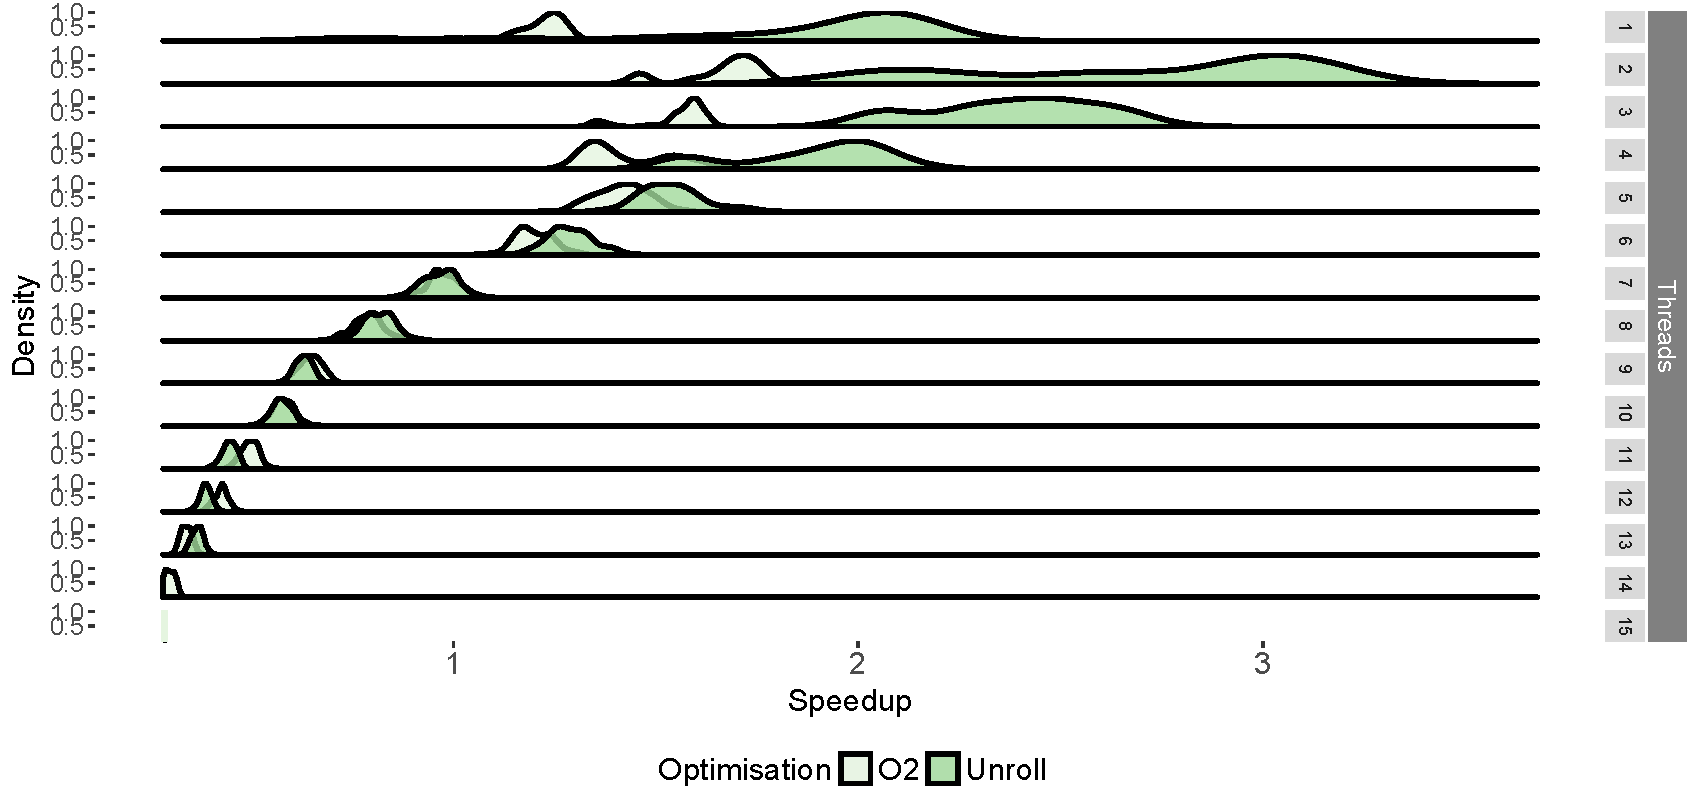
\includegraphics[width=1\textwidth]{streamit-paper/graphics/appendixgraphs/fft6-total2.pdf}
\caption{FFT6}\label{chp:stream:f6t}
\end{figure}
\begin{figure}[t]
\center
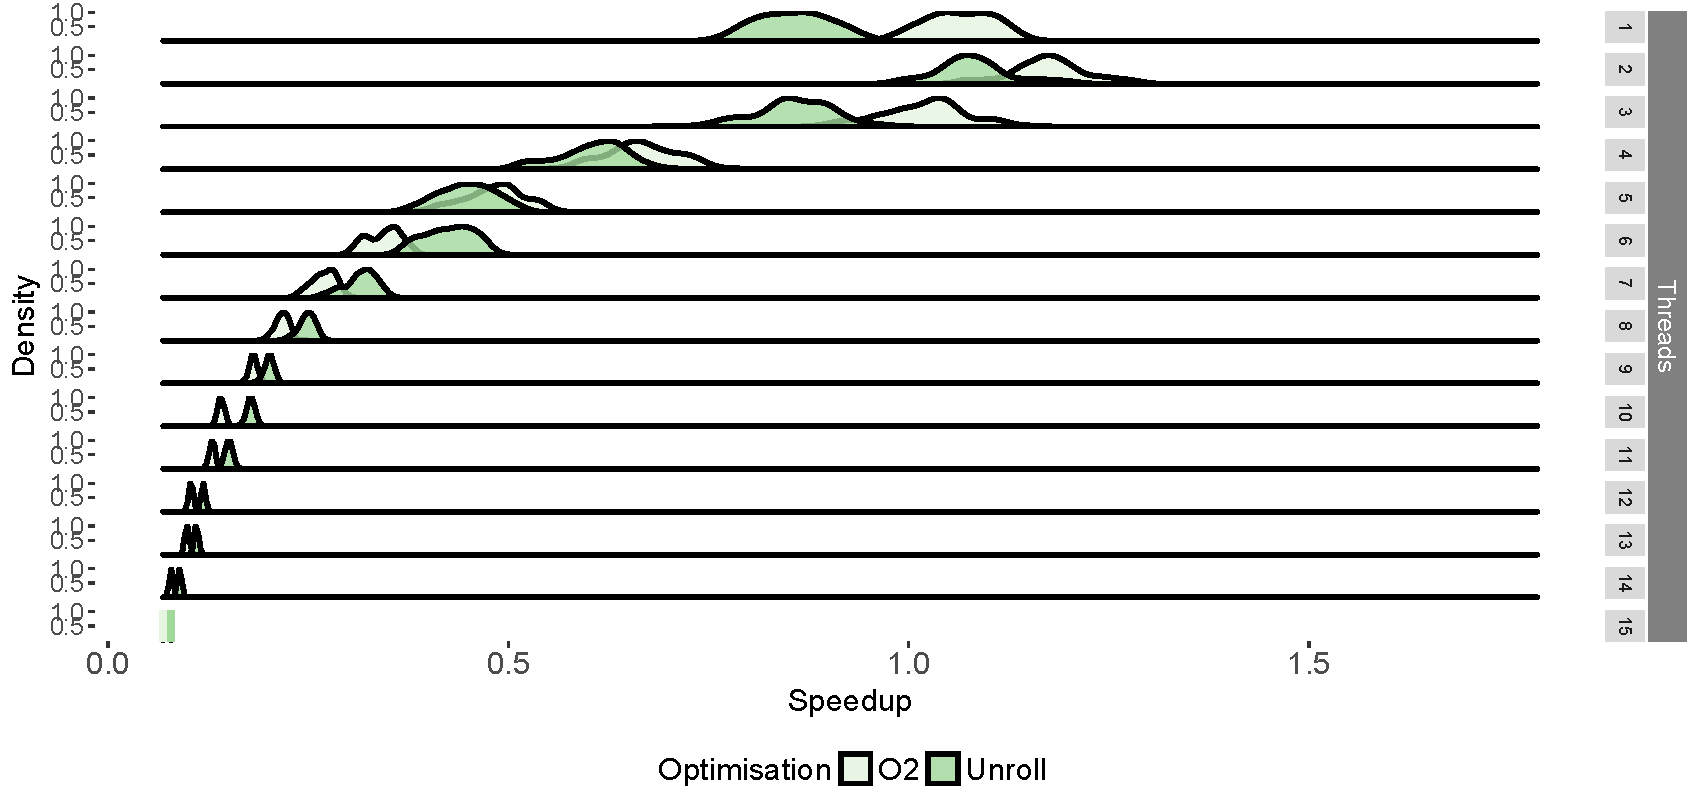
\includegraphics[width=1\textwidth]{streamit-paper/graphics/appendixgraphs/fir-total2.pdf}
\caption{FIR}\label{chp:stream:fit}
\center
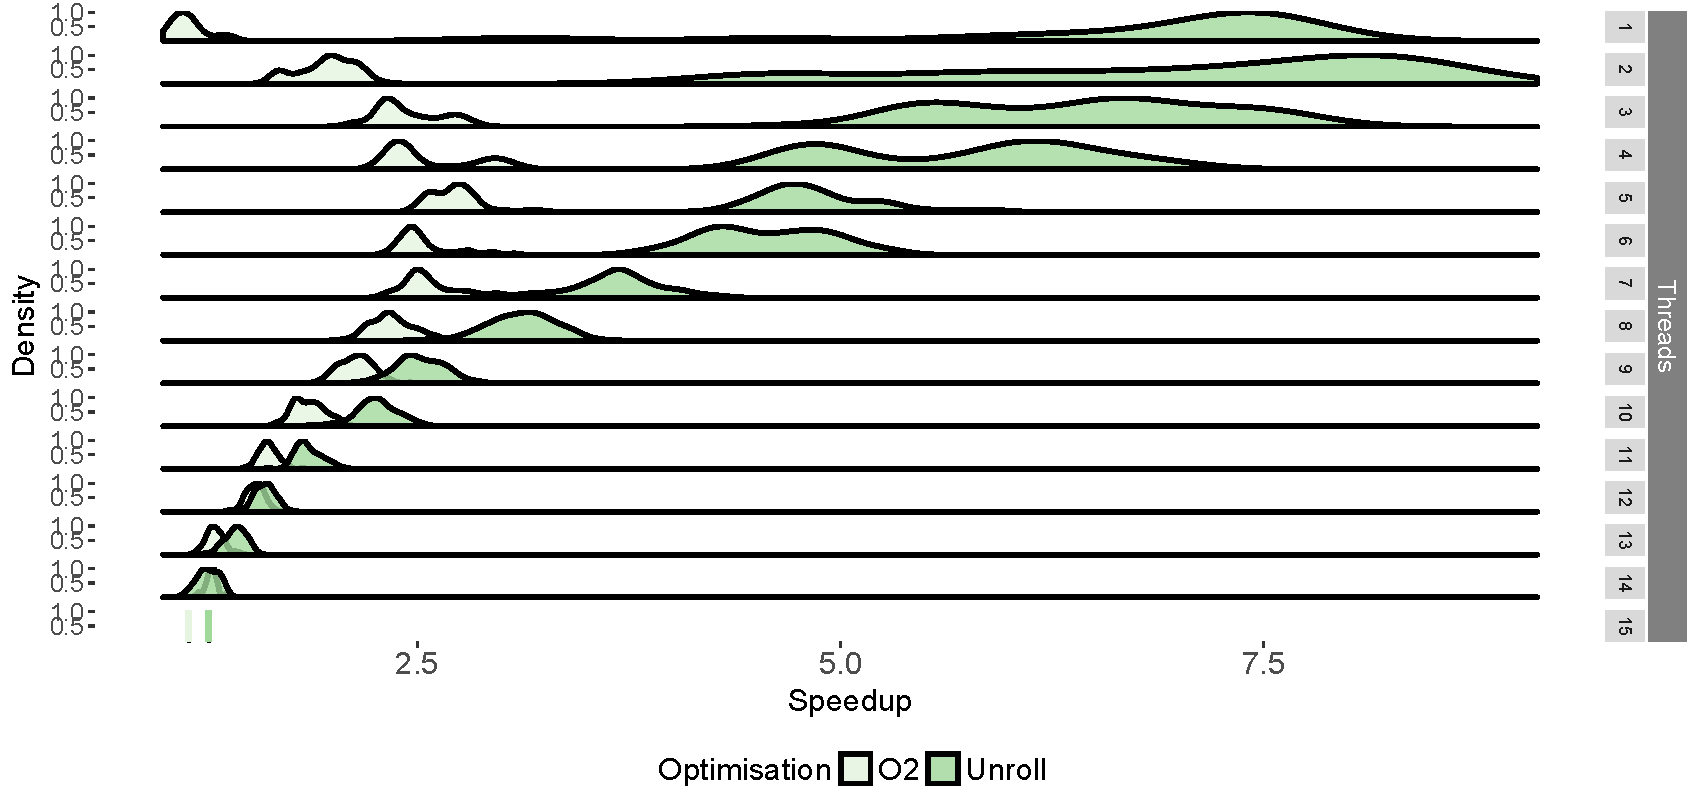
\includegraphics[width=1\textwidth]{streamit-paper/graphics/appendixgraphs/fm-total2.pdf}
\caption{FMRadio}\label{chp:stream:fmt}
\center
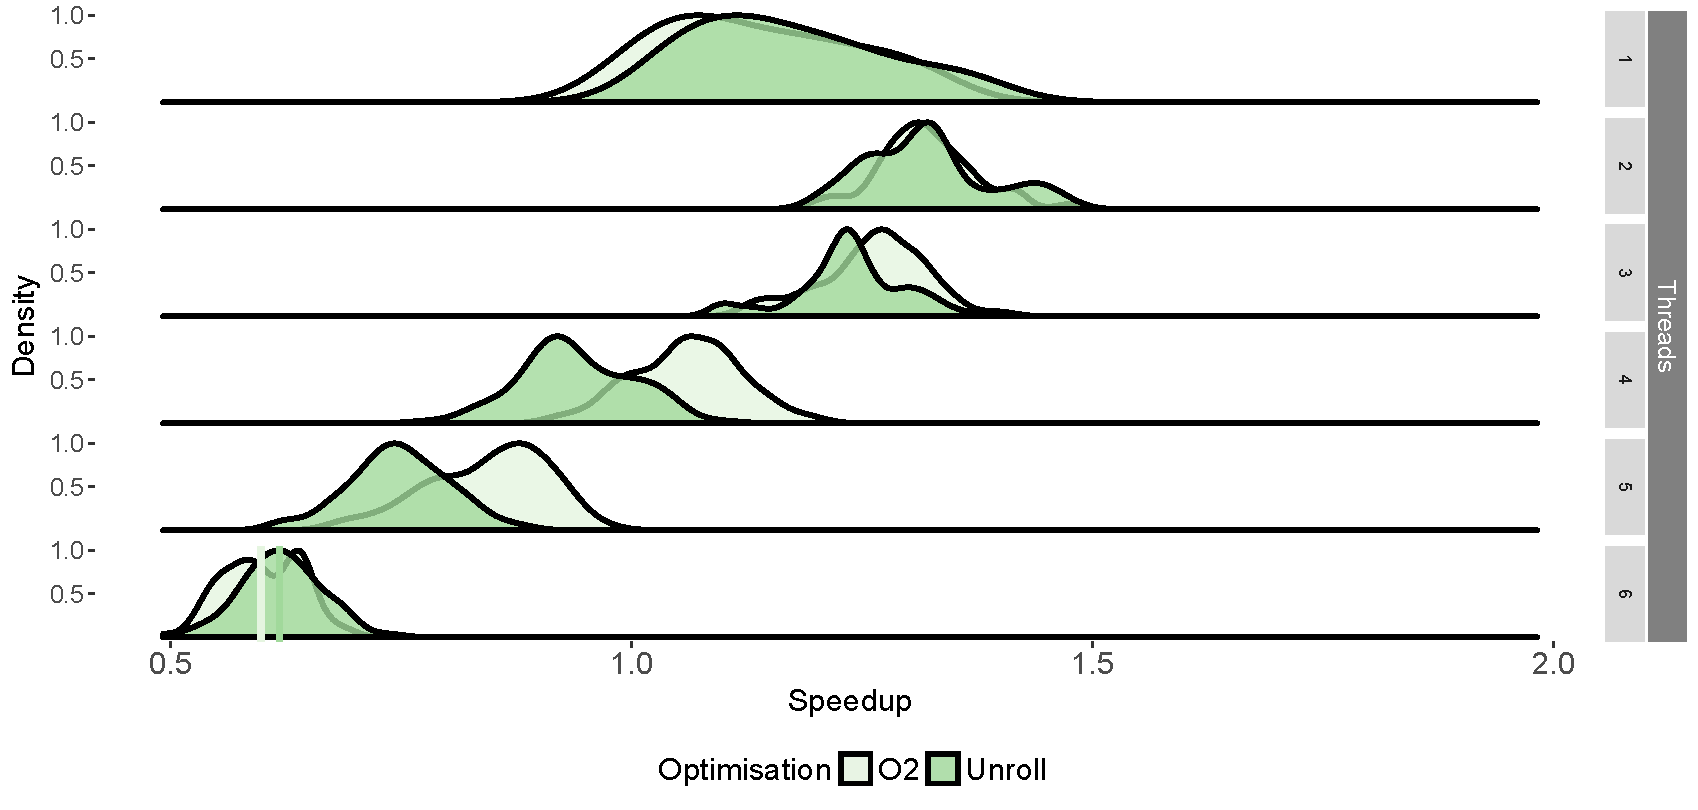
\includegraphics[width=1\textwidth]{streamit-paper/graphics/appendixgraphs/insertion-total2.pdf}
\caption{Insertion}\label{chp:stream:it}

\end{figure}
\begin{figure}[t]
\center
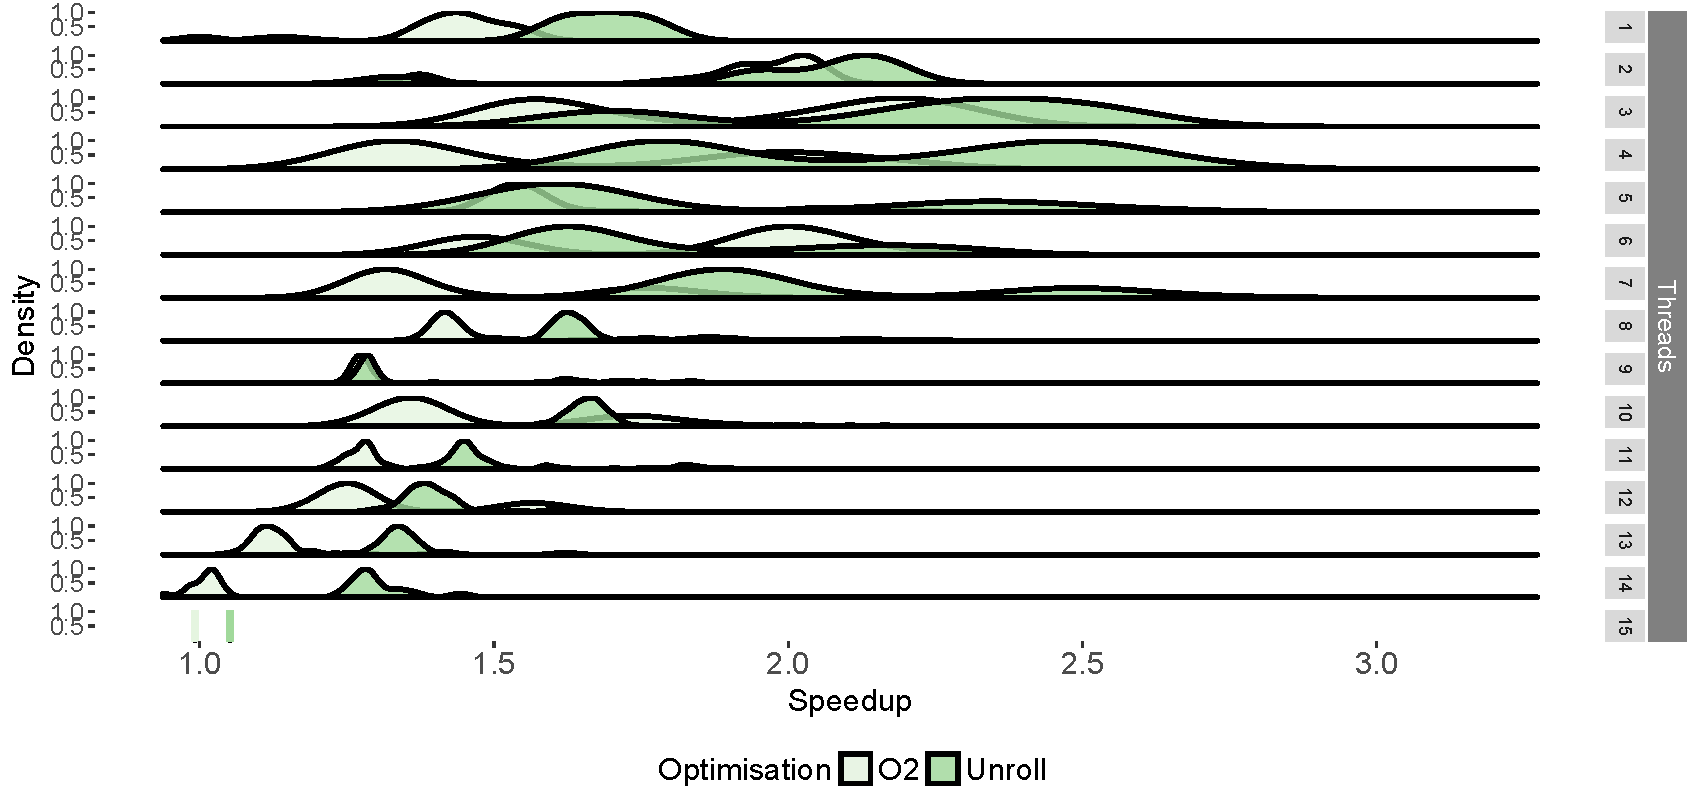
\includegraphics[width=1\textwidth]{streamit-paper/graphics/appendixgraphs/matmul-total2.pdf}
\caption{Matmul}\label{chp:stream:mt}
 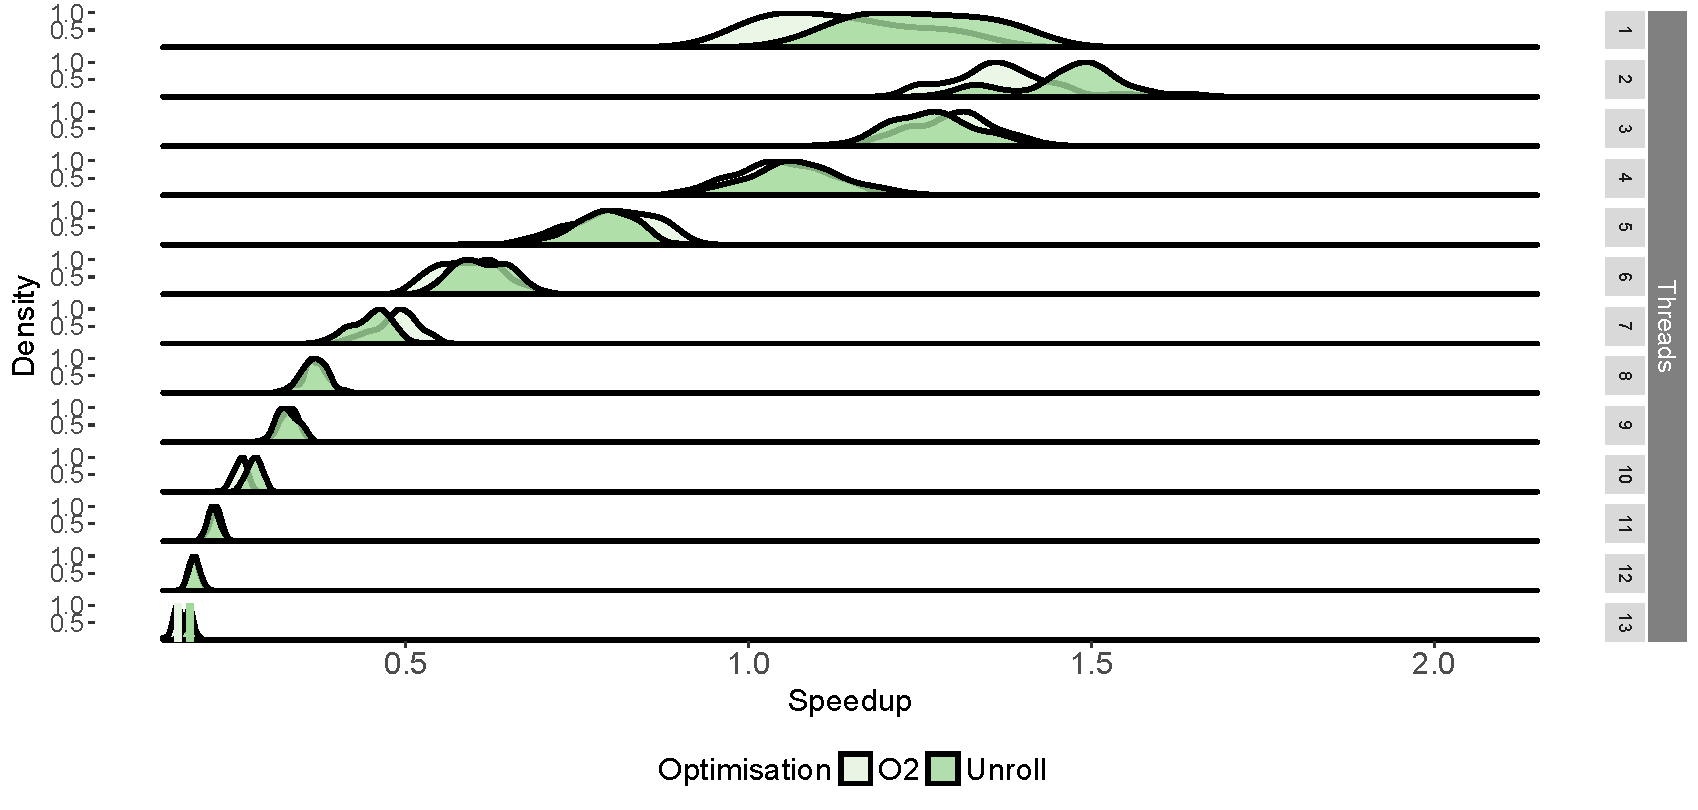
\includegraphics[width=1\textwidth]{streamit-paper/graphics/appendixgraphs/radix-total2.pdf}
\caption{Radix}\label{chp:stream:rt}
\end{figure} 

\FloatBarrier
\chapter{Dynamic runtime adaptation for efficient execution}

\section{Code listings}

\lstset{
	backgroundcolor=\color{lbcolor},
	tabsize=2,
	rulecolor=,
	language=matlab,
        basicstyle=\tiny,
        upquote=true,
        aboveskip={1\baselineskip},
        columns=fixed,
        showstringspaces=false,
        extendedchars=true,
        breaklines=true,
        prebreak = \raisebox{0ex}[0ex][0ex]{\ensuremath{\hookleftarrow}},
        frame=single,
        showtabs=false,
        showspaces=false,
        showstringspaces=false,
        identifierstyle=\ttfamily,
        keywordstyle=\color[rgb]{0,0,1},
        commentstyle=\color[rgb]{0.133,0.545,0.133},
        stringstyle=\color[rgb]{0.627,0.126,0.941},
		numbers=left,
}

\begin{lstlisting}[language=C,basicstyle=\small]
int ndims = 2;
for(i = 0 ; i < nel ; ++i) {
	idx_t index = pairs_pt [i].index ;    
	val_t value = pairs_pt [i].value ;
	rindex = index ;
	forest_pt [index] .parent   = index ;
	forest_pt [index] .shortcut = index ;
	forest_pt [index] .area     = 1 ;
	idx_t temp = index ;
	for(k = ndims-1 ; k >=0 ; --k) {
		sref(nsubs_pt,k) = -1 ;
		sref(subs_pt,k) = temp / sref(strides_pt,k) ;
		temp         = temp % sref(strides_pt,k) ;
	}
	while(1) {
		int good = 1 ;
		idx_t nindex = 0 ;
		for(k = 0 ; k < ndims && good ; ++k) {
			int temp = sref(nsubs_pt,k) + sref(subs_pt,k) ;
			good &= 0 <= temp && temp < sref(dims,k) ;
			nindex += temp * sref(strides_pt,k) ;
		}
		if(good && nindex != index && forest_pt[nindex].parent != node_is_void ) {
			idx_t nrindex = 0, nvisited ;
			val_t nrvalue = 0 ;
			nvisited = 0 ;
			while( forest_pt[rindex].shortcut != rindex ) {          
				sref(visited_pt,nvisited++) = rindex ;
				rindex = forest_pt[rindex].shortcut ;
			}      
			while( nvisited-- ) {
				forest_pt [ sref(visited_pt,nvisited) ] .shortcut = rindex ;
			}
			nrindex  = nindex ;
			nvisited = 0 ;
			while( forest_pt[nrindex].shortcut != nrindex ) {          
				sref(visited_pt, nvisited++) = nrindex ;
				nrindex = forest_pt[nrindex].shortcut ;
			}      
			while( nvisited-- ) {
				forest_pt [ sref(visited_pt,nvisited) ] .shortcut = nrindex ;
			}
			if( rindex != nrindex ) {
				nrvalue = asubsref(I_pt,nrindex) ;
				if( nrvalue == value) {
					forest_pt[rindex] .parent   = nrindex ;
					forest_pt[rindex] .shortcut = nrindex ;          
					forest_pt[nrindex].area    += forest_pt[rindex].area ;
					sref(joins_pt,njoins++) = rindex ;
				} 
				else {
					forest_pt[nrindex] .parent   = rindex ;
					forest_pt[nrindex] .shortcut = rindex ;
					forest_pt[rindex]  .area    += forest_pt[nrindex].area ;
					if( nrvalue != value ) {            
						forest_pt[nrindex].region = ner ;
						regions_pt [ner] .index      = nrindex ;
						regions_pt [ner] .parent     = ner ;
						regions_pt [ner] .value      = nrvalue ;
						regions_pt [ner] .area       = forest_pt [nrindex].area ;
						regions_pt [ner] .area_top   = nel ;
						regions_pt [ner] .area_bot   = 0 ;            
						++ner ;
					}
					sref(joins_pt,njoins++) = nrindex ;
				}
			}
		}
		k = 0 ;
		sref(nsubs_pt,k) = sref(nsubs_pt,k) + 1;
		while( sref(nsubs_pt, k) > 1) {
			sref(nsubs_pt,k++) = -1 ;
			if(k == ndims) goto done_all_neighbors ;
			sref(nsubs_pt,k) = sref(nsubs_pt,k) + 1;
		}
	}
	done_all_neighbors : ;
}

\end{lstlisting}
\newpage
\captionof{lstlisting}{MSER Compute extremal regions tree source code}\label{lsting:mser}

\begin{lstlisting}[language=C,basicstyle=\small]
I2D* fSortIndices(F2D* input, int dim)
{
    int rows, cols;
    F2D *in;
    int i, j, k;
    I2D *ind;

    rows = input->height;
    cols = input->width;
    in = fDeepCopy(input);
    ind = iMallocHandle(rows,cols);

    for(i=0; i<cols; i++)
        for(j=0; j<rows; j++)
            subsref(ind,j,i) = 0;

    for(k=0; k<rows; k++) {
        for(i=0; i<cols; i++) {
            float localMax = subsref(in,k,i);
            int localIndex = i;
            subsref(ind,k,i) = i;
            for(j=0; j<cols; j++) {
                if(localMax < subsref(in,k,j)) {
                    subsref(ind,k,i) = j;
                    localMax = subsref(in,k,j);
                    localIndex = j;
                }
            }
            subsref(in,k,localIndex) = 0;
        }
    }
    fFreeHandle(in);
    return ind;
}

int find(universe* u, int x) {
    int y=x;
    while (y != u->elts[y].p)
        y = u->elts[y].p;
    u->elts[x].p = y;
    return y;
}

void join(universe* u, int x, int y){
    if (u->elts[x].rank > u->elts[y].rank) {
        u->elts[y].p = x;
        u->elts[x].size += u->elts[y].size;
    } 
    else {
        u->elts[x].p = y;
        u->elts[y].size += u->elts[x].size;
        if (u->elts[x].rank == u->elts[y].rank)
            u->elts[y].rank++;
    }
    u->num--;
    return ;
}

universe *segment_graph(int num_vertices, int num_edges, edge *edges, float c) { 
    float* threshold = alloca(sizeof(int) * num_vertices);
    int i, a, b, j, k;
    universe *u;
    F2D *edgeWeig!htbs;
    I2D *indices;
    edgeWeig!htbs = fMallocHandle(1,num_edges);

    for(i=0; i<num_edges; i++)
        asubsref(edgeWeig!htbs,i) = edges[i].w;

    indices = fSortIndices(edgeWeig!htbs,1);
    u = (universe*)malloc(sizeof(universe));
    u->elts = (uni_elt*)malloc(sizeof(uni_elt)*num_vertices);
    u->num = num_vertices;
	
    for(i=0; i<num_vertices; i++)    {
        u->elts[i].rank = 0;
        u->elts[i].size = 1;
        u->elts[i].p = i;
    }

    for (i = 0; i < num_vertices; i++)
        arrayref(threshold,i) = THRESHOLD(1,c);

    for (i = 0; i < num_edges; i++) {
        edge *pedge = &edges[ asubsref(indices,i) ];
		a = find(u, pedge->a);
        b = find(u, pedge->b);
        if (a != b) {
            if ((pedge->w <= arrayref(threshold,a)) && (pedge->w <= arrayref(threshold,b))) {
	            join(u, a, b);
	            a = find(u, a);
	            arrayref(threshold,a) = pedge->w + THRESHOLD(u->elts[a].size, c);
            }
        }
    }
  return u;
}
\end{lstlisting}
\captionof{lstlisting}{Multi\_NCut main phase of segmenting image}\label{lsting:multi}
\end{appendices}